% Hlavicka pro protokoly z fyzikalniho praktika.
% Verze pro: LaTeX
% Verze hlavicky: 22. 2. 2007
% Autor: Ustav fyziky kondenzovanych latek
% Ke stazeni: www.physics.muni.cz/ufkl/Vyuka/
% Licence: volne k pouziti, nejlepe k vcasnemu odevzdani protokolu z Vaseho mereni.


\documentclass[czech,11pt,a4paper]{article}
\usepackage[T1]{fontenc}
\usepackage{graphicx, animate}
\usepackage{mathtools}
\usepackage{amssymb}
\usepackage{amsthm}
\usepackage{thmtools}
\usepackage{xcolor}
\usepackage{nameref}
\usepackage{babel}
\usepackage{hyperref}
\usepackage{multicol}
\usepackage[export]{adjustbox}
\usepackage{subcaption}
\usepackage{caption}
\usepackage{multirow}
\usepackage{float}
\usepackage{placeins}
\usepackage{biblatex}
\graphicspath{ {./images/} }




%%% Nemente:
\usepackage[margin=2cm]{geometry}
\newtoks\jmenopraktika \newtoks\jmeno \newtoks\datum
\newtoks\obor \newtoks\skupina \newtoks\rocnik \newtoks\semestr
\newtoks\cisloulohy \newtoks\jmenoulohy
\newtoks\tlak \newtoks\teplota \newtoks\vlhkost
%%% Nemente - konec.


%%%%%%%%%%% Doplnte pozadovane polozky:

\jmenopraktika={Fyzikální praktikum 2}  % nahradte jmenem vaseho predmetu
\jmeno={Teodor Duraković}            % nahradte jmenem mericiho
\datum={2.~prosince 2024}        % nahradte datem mereni ulohy
\obor={F}                     % nahradte zkratkou vami studovaneho oboru
\skupina={Po 14:00}            % nahradte dobou vyuky vasi seminarni skupiny
\rocnik={II}                  % nahradte rocnikem, ve kterem studujete
\semestr={III}                 % nahradte semestrem, ve kterem studujete

\cisloulohy={8}               % nahradte cislem merene ulohy
\jmenoulohy={Měření parametrů zobrazovacích soustav} % nahradte jmenem merene ulohy

\tlak={994}                   % nahradte tlakem pri mereni (v hPa)
\teplota={21.6}               % nahradte teplotou pri mereni (ve stupnich Celsia)
\vlhkost={33}               % nahradte vlhkosti vzduchu pri mereni (v %)

%%%%%%%%%%% Konec pozadovanych polozek.


%%%%%%%%%%% Uzitecne balicky:

%%%%%% Zamezeni parchantu:
\widowpenalty 10000 \clubpenalty 10000 \displaywidowpenalty 10000
%%%%%% Parametry pro moznost vsazeni vetsiho poctu obrazku na stranku
\setcounter{topnumber}{3}	  % max. pocet floatu nahore (specifikace t)
\setcounter{bottomnumber}{3}	  % max. pocet floatu dole (specifikace b)
\setcounter{totalnumber}{6}	  % max. pocet floatu na strance celkem
\renewcommand\topfraction{0.9}	  % max podil stranky pro floaty nahore
\renewcommand\bottomfraction{0.9} % max podil stranky pro floaty dole
\renewcommand\textfraction{0.1}	  % min podil stranky, ktery musi obsahovat text
\intextsep=8mm \textfloatsep=8mm  %\intextsep pro ulozeni [h] floatu a \textfloatsep pro [b] or [t]

% Tecky za cisly sekci:
\renewcommand{\thesection}{\arabic{section}.}
\renewcommand{\thesubsection}{\thesection\arabic{subsection}.}
\renewcommand{\thesubsubsection}{\thesubsection\arabic{subsubsection}.}
% Jednopismenna mezera mezi cislem a nazvem kapitoly:
\makeatletter \def\@seccntformat#1{\csname the#1\endcsname\hspace{1ex}} \makeatother


%%%%%%%%%%%%%%%%%%%%%%%%%%%%%%%%%%%%%%%%%%%%%%%%%%%%%%%%%%%%%%%%%%%%%%%%%%%%%%%
%%%%%%%%%%%%%%%%%%%%%%%%%%%%%%%%%%%%%%%%%%%%%%%%%%%%%%%%%%%%%%%%%%%%%%%%%%%%%%%
% Zacatek dokumentu
%%%%%%%%%%%%%%%%%%%%%%%%%%%%%%%%%%%%%%%%%%%%%%%%%%%%%%%%%%%%%%%%%%%%%%%%%%%%%%%
%%%%%%%%%%%%%%%%%%%%%%%%%%%%%%%%%%%%%%%%%%%%%%%%%%%%%%%%%%%%%%%%%%%%%%%%%%%%%%%

\begin{document}
	
	%%%%%%%%%%%%%%%%%%%%%%%%%%%%%%%%%%%%%%%%%%%%%%%%%%%%%%%%%%%%%%%%%%%%%%%%%%%%%%%
	% Nemente:
	%%%%%%%%%%%%%%%%%%%%%%%%%%%%%%%%%%%%%%%%%%%%%%%%%%%%%%%%%%%%%%%%%%%%%%%%%%%%%%%
	\thispagestyle{empty}
	
	{
		\begin{center}
			\sf 
			{\Large Ústav fyzikální elektroniky Přírodovědecké fakulty Masarykovy univerzity} \\
			\bigskip
			{\huge \bfseries FYZIKÁLNÍ PRAKTIKUM} \\
			\bigskip
			{\Large \the\jmenopraktika}
		\end{center}
		
		\bigskip
		
		\sf
		\noindent
		\setlength{\arrayrulewidth}{1pt}
		\begin{tabular*}{\textwidth}{@{\extracolsep{\fill}} l l}
			\large {\bfseries Zpracoval:}  \the\jmeno & \large  {\bfseries Naměřeno:} \the\datum\\[2mm]
			\large  {\bfseries Obor:} \the\obor  \hspace{40mm}  {\bfseries Skupina:} \the\skupina %
			%{\bfseries Ročník:} \the\rocnik \hspace{5mm} {\bfseries Semestr:} \the\semestr  
			&\large {\bfseries Testováno:}\\
			\\
			\hline
		\end{tabular*}
	}
	
	\bigskip
	
	{
		\sf
		\noindent \begin{tabular}{p{3cm} p{0.6\textwidth}}
			\Large  Úloha č. {\bfseries \the\cisloulohy:} \par
			\smallskip
			$T=\the\teplota$~$^\circ$C \par
			$p=\the\tlak$~hPa \par
			$\varphi=\the\vlhkost$~\%
			&\Large \bfseries \the\jmenoulohy  \\[2mm]
		\end{tabular}
	}
	
	\vskip1cm
	
	%%%%%%%%%%%%%%%%%%%%%%%%%%%%%%%%%%%%%%%%%%%%%%%%%%%%%%%%%%%%%%%%%%%%%%%%%%%%%%%
	% konec Nemente.
	%%%%%%%%%%%%%%%%%%%%%%%%%%%%%%%%%%%%%%%%%%%%%%%%%%%%%%%%%%%%%%%%%%%%%%%%%%%%%%%
	
	%%%%%%%%%%%%%%%%%%%%%%%%%%%%%%%%%%%%%%%%%%%%%%%%%%%%%%%%%%%%%%%%%%%%%%%%%%%%%%%
	%%%%%%%%%%%%%%%%%%%%%%%%%%%%%%%%%%%%%%%%%%%%%%%%%%%%%%%%%%%%%%%%%%%%%%%%%%%%%%%
	% Zacatek textu vlastniho protokolu
	%%%%%%%%%%%%%%%%%%%%%%%%%%%%%%%%%%%%%%%%%%%%%%%%%%%%%%%%%%%%%%%%%%%%%%%%%%%%%%%
	%%%%%%%%%%%%%%%%%%%%%%%%%%%%%%%%%%%%%%%%%%%%%%%%%%%%%%%%%%%%%%%%%%%%%%%%%%%%%%%
	
	\begin{multicols}{2}
		\section{Zadání}
		1. Změřit ohniskovou vzdálenost tenké spojky\\
		2. Změřit ohniskovou vzdálenost tenké rozptylky\\
		3. Určit index lomu čoček z ohniskové vzdálenosti a měření křivosti
		\section*{Měření odrazivosti dielektrika}
	Průchod paraxiálních paprsků soustavou centrovaných kulových lámavých ploch je popsán zakladními zobrazovacími parametry, mezi než patří hlavní a uzlové body (respektive roviny), ohniska a ohniskové vzdálenosti. Dopadá-li na zobrazovací soustavu (obr. 1) svazek paprsků rovnoběžných s optickou osou $O$, pak po průchodu soustavou se paprsky protínají v obrazovém ohnisku $F^{\prime}$. Naopak, svazek paprsků vycházejících z bodu $F$ (předmětové ohnisko) se změní po průchodu soustavou na rovnoběžný svazek. Rovina kolmá k optické ose procházející předmětovým, respektive obrazovým ohniskem se nazývá předmětovou, respektive obrazovou ohniskovou rovinou. Na obr. 1 jsou obrazem bodů $A, B$ body $A^{\prime}, B^{\prime}$. Poměr úseček $y^{\prime}=A^{\prime} B^{\prime}$ a $y=A B$ se nazývá příčným zvětšením $\beta$,
	
	\begin{equation}
		\beta=\frac{y^{\prime}}{y} .
	\end{equation}
	
	
	Poměr úhlů $\alpha^{\prime}$ a $\alpha$, které svíraji sdružené paprsky procházející ohnisky s optickou osou, se nazývá úhlové zvětšení $\gamma$,
	\begin{equation}
		\gamma=\frac{u^{\prime}}{u}
	\end{equation}
	
	
	Hlavními rovinami $H$ a $H^{\prime}$ soustavy nazýváme dvojici sdružených rovin, kolmých k optické ose, pro než je příčné zvětšení rovno jedné. Hlavními body nazýváme průsečíky hlavních rovin s optickou osou.
\begin{figure}[H]

		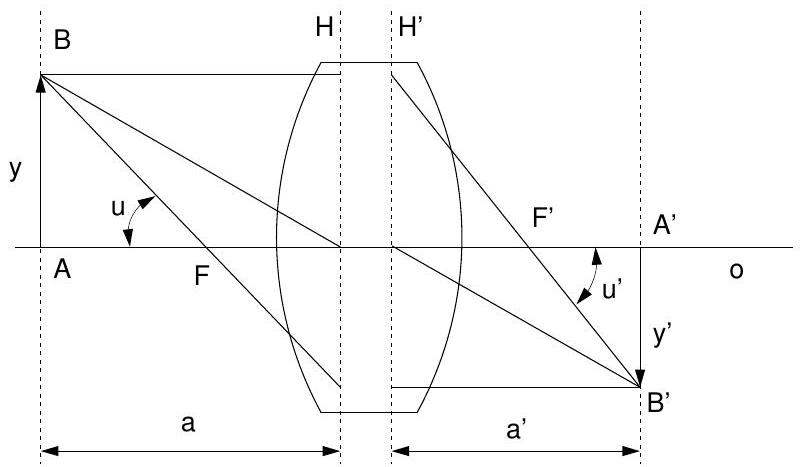
\includegraphics[max width=0.95\linewidth, center]{2024_12_03_2b013636ff75d184213cg-1}

	
	\caption{Zobrazení pomocí zobrazovací soustavy. Hlavní roviny čočky jsou označeny $H$ a $H^{\prime}$, ohniska $F$ a $F^{\prime}, A B$ je předmět a $A^{\prime} B^{\prime}$ obraz.\\
	}

		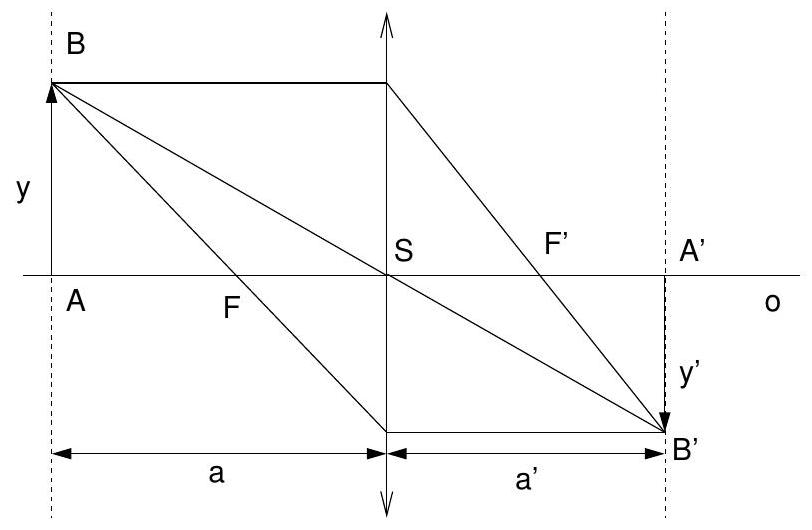
\includegraphics[max width=0.95\linewidth,center]{2024_12_03_2b013636ff75d184213cg-2}
		\caption{Přímé měření ohniskové vzdálenosti tenké čočky}
\end{figure}

Je-li tlouštka čočky zanedbatelná ve srovnání s poloměry křivosti lámavých ploch, hovoříme o tenké čočce. V takovém případě hlavní roviny $H$ a $H^{\prime}$ splývají a čočka je pak při výpočtech představována rovinou středního řezu.

\section{Znaménková konvence a zobrazovací rovnice tenké čočky}

Předmětový a obrazový prostor jsou charakterizovány souřadnými soustavami, jejichž počátky v případě tenké čočky leží ve stejném bodě ve středu čočky. Při výpočtech je nutné rozlišovat kladné a záporné hodnoty v těchto souřadných soustavách. Definice kladného a záporného prostoru může být různá, avšak je-li zvolená určitá definice, všechny vztahy musí být v souhlasu s touto konvencí. Budeme důsledně používat následující znaménkovou konvenci: vzdálenost měříme od středu čočky a sice tak, že leží-li bod napravo od počátku bereme vzdálenosti kladně a v opačném případě záporně; leží-li bod nad osou $O$ bereme vzdálenosti kladně a v opačném případě záporně. Na obr. 2 je znázorněno zobrazování spojkou - vidíme, že tady $a<0, a^{\prime}>0, f<0, f^{\prime}>0$, $y>0$ a $y^{\prime}<0$. V uvedené znaménkové konvenci zobrazovací rovnice čočky má tvar
\begin{equation}
	\frac{1}{a^{\prime}}-\frac{1}{a}=\frac{1}{f^{\prime}}
\end{equation}

kde $a$ je předmětová vzdálenost, $a^{\prime}$ je obrazová vzdálenost a $f^{\prime}$ je obrazová ohnisková vzdálenost.

\section{Stanovení ohniskové vzdálenosti tenké spojky z polohy obrazu a předmětu}

Ze zobrazovací rovnice (3) vyplývá pro ohniskovou vzdálenost $f^{\prime}$ vztah

\begin{equation}
	f^{\prime}=\frac{a a^{\prime}}{a-a^{\prime}}
\end{equation}


Určíme-li tedy vzdálenosti $a$ a $a^{\prime}$, pak pomocí vztahu 4 vypočítame $f^{\prime}$. Měření se provádí na optické lavici s měřítkem, na které je umístěn předmět $y$ (svítící šipka s vestavěným měřitkem), studovaná čočka $S$ a stínítko, na něž zachycujeme obraz $y^{\prime}$ (viz obr. 2). Změnou polohy čočky nebo stínítka při stálé poloze předmětu hledáme co nejlépe zaostřený obraz a odečteme na měřítku optické lavice hodnoty $a, a^{\prime}$.

\section*{Stanovení ohniskové vzdálenosti tenké čočky z příčného zvětšení}

Pro přičné zvětšení platí

\begin{equation}
	\beta=\frac{y^{\prime}}{y}=\frac{a^{\prime}}{a} .
\end{equation}

\begin{figure}[H]
	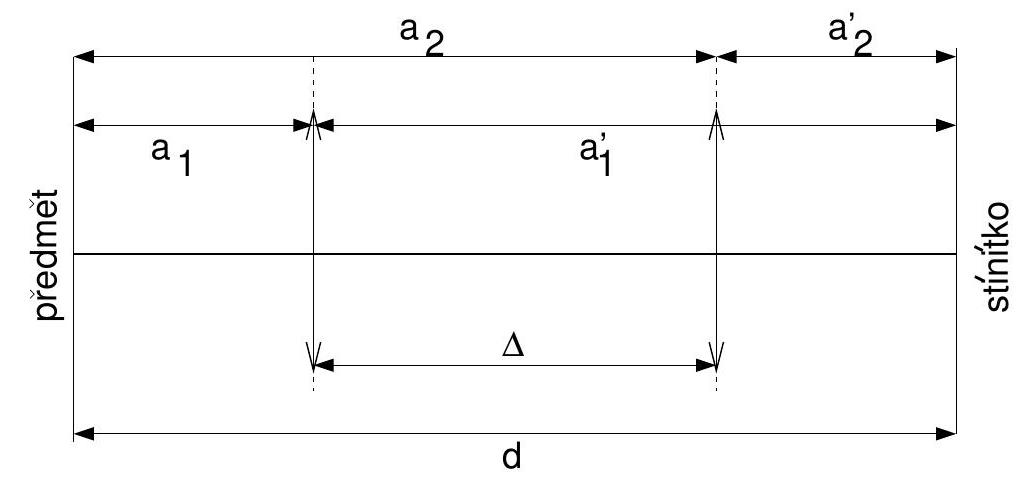
\includegraphics[width = 0.95\linewidth, center]{2024_12_03_2b013636ff75d184213cg-3}
	\caption{Besselova metoda měření ohniskové vzdálenosti.}
\end{figure}
Rovnici (8.4) přepíšeme do tvaru

\begin{equation}
	f^{\prime}=\frac{a^{\prime}}{1-\beta}=\frac{a \beta}{1-\beta}
\end{equation}


Zvětšení $\beta$ určíme tak, že na stínítku změříme určitou část osvětleného milimetrového měřítka. K změřenému $\beta$ přířadíme odpovídající vzdálenost $a$ nebo $a^{\prime}$. Z rovnice 6) vypočítame ohniskovou vzdálenost. Z hlediska dosažení maximální přesnosti je vhodné volit vzdálenost $a$ co největší, na druhé straně bereme zřetel na to, aby obraz byl dostatečně velký, aby zvětšení bylo dobře měřitelné.

\section*{Stanovení ohniskové vzdálenosti tenké spojky Besselovou metodou}

Uvažujeme uspořádání podle obr. 3. Vzdálenost $d$ předmětu od stínítka ponecháme pevnou. Dá se ukázat, že pro $d>4 f$ existují dvě polohy spojky, ve kterých se na stínítku vytvoří ostrý obraz. Vzhledem k tomu, že polohy předmětu a obrazu mohou být vzájemně vyměněny,
\begin{equation}
	a_{1}=-a_{2}^{\prime}, \quad a_{2}=-a_{1}^{\prime}
\end{equation}

a dále platí (viz.obr. 8.3)

\begin{align}
	& d=\left|a_{1}\right|+\left|a_{1}^{\prime}\right|=\left|a_{2}\right|+\left|a_{2}^{\prime}\right| \\
	& \Delta=\left|a_{1}^{\prime}\right|-\left|a_{2}^{\prime}\right|=\left|a_{2}\right|-\left|a_{1}\right| .
\end{align}


Pak ze vztahů 8.7- 8.9 lze odvodit, že
\begin{equation}
	d^{2}-\Delta^{2}=4 a_{1} a_{1}^{\prime}=4 a_{2} a_{2}^{\prime}
\end{equation}


Dosadíme-li do vztahu 8.4 za čitatele $a a^{\prime}$ ze vztahu 8.10 a za jmenovatele $d$ ze vztahu 8.8, dostaneme vztah pro určení ohniskové vzdálenosti
\begin{equation}
	f^{\prime}=\frac{d^{2}-\Delta^{2}}{4 d}
\end{equation}


\section*{Stanovení ohniskové vzdálenosti tenké rozptylky}

Rozptylky vytvářejí vždy neskutečný obraz skutečného předmětu nebo naopak skutečný obraz neskutečného předmětu. Proto je v tomto případě nutno postupovat tak, že k měřené rozptylce se přidá spojka tak, aby obraz vytvořený spojkou mohl být neskutečným předmětem pro rozptylku. Podle obr. 4 umístíme na optickou lavici předmět $y_{s}$, a spojkou $S$ vytvoříme reálný obraz $y_{s}^{\prime}$, v bodě $A$. Mezi tento obraz a spojku umístíme rozptylku $R$ a na stínítku zase nalezneme ostrý obraz $y_{r}^{\prime}$ v bodě $A^{\prime}$. Obraz $y_{s}^{\prime}$ je vlastně předmětem $y_{r}$ pro rozptylku. Známe-li polohu rozptylky $R$, polohu obrazu spojky $A$ a polohu obrazu roztylky $A^{\prime}$, můžeme vypočítat
\begin{equation}
	a=A-R \quad a^{\prime}=A^{\prime}-R
\end{equation}

a pro výpočet ohniskové vzdálenosti rozptylky použít vztah (8.4).
\begin{figure}[H]
	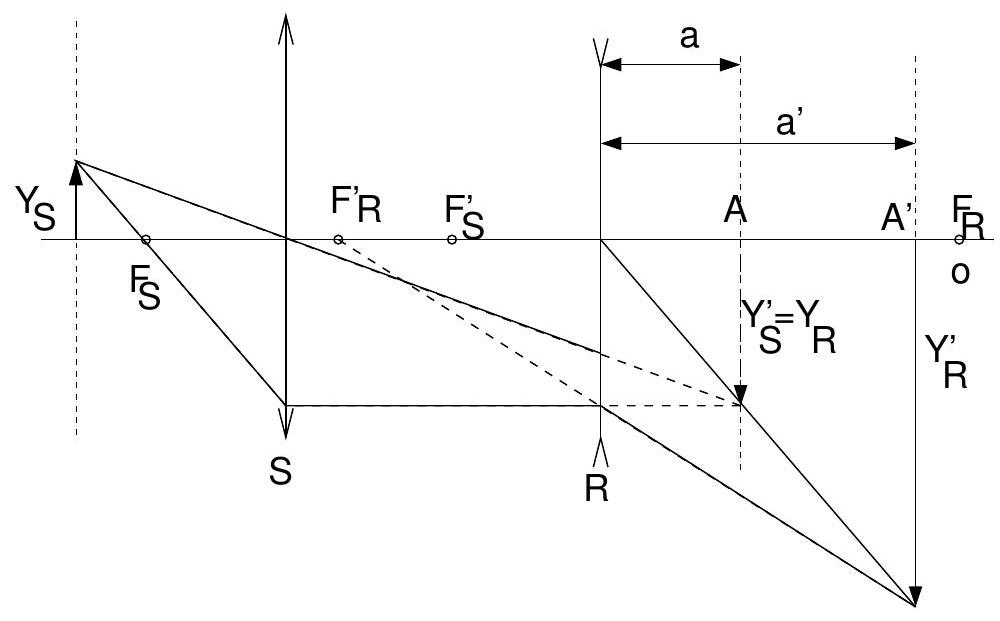
\includegraphics[width = 0.95\linewidth, center]{2024_12_03_2b013636ff75d184213cg-4}
	\caption{Měření ohniskové vzdálenosti rozptylky.}
\end{figure}

\section*{Určení indexu lomu čoček z ohniskové vzdálenosti a měření křivosti}
\begin{figure}[H]
	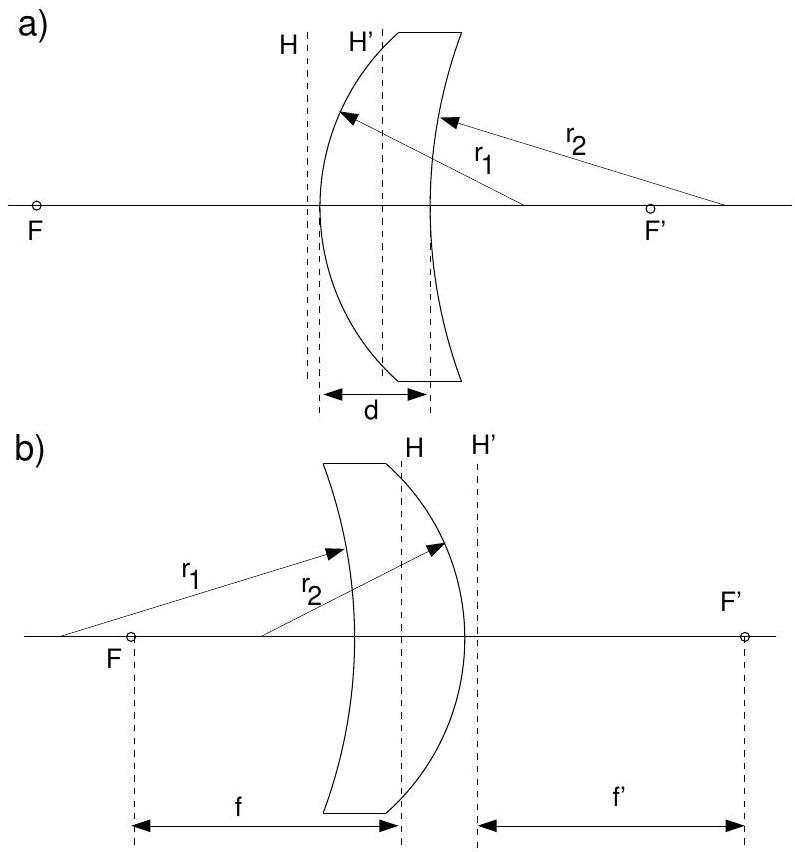
\includegraphics[width = 0.95\linewidth, center]{2024_12_03_2b013636ff75d184213cg-5}
	\caption{Základní parametry tlusté čočky.}
\end{figure}


Index lomu určíme ze vztahu [3]
\begin{equation}
	\frac{1}{f^{\prime}}=(n-1)\left(\frac{1}{r_{1}}-\frac{1}{r_{2}}\right)+\frac{d(n-1)^{2}}{n r_{1} r_{2}}
\end{equation}

kde $f^{\prime}$ je ohnisková vzdálenost, $r_{1}, r_{2}$ poloměry kulových ploch, $n$ index lomu a $d$ tloušťka čočky. Na obr. 5 jsou vyznačeny tyto parametry pro různé polohy čočky. Vztah 8.13 předpokládá použití znaménkové konvence, která je popsaná v předchozí části.

Obrázek 5 představuje tlustou spojnou čočku s jednou stranou vypuklou a druhou vydutou, která se často používá v brýlové optice. Na obr. 5 jsou uvedeny dvě polohy stejné čočky, kdy $r_{1}>0$ a $r_{2}>0$ (schéma (a)) a $r_{1}<0$ a $r_{2}<0$ (schéma (b)). V obecném případě se můžeme setkat


s čočkami s oběma stranami vypuklými či oběma vydutými, případně s jednou stranou ploskou. V každém případě se však držíme znaménkové konvence, ve které je znaménko poloměru křivosti bylo záporné je-li střed křivosti plochy nalevo od vrcholu čočky a kladné v opačném případě. Pro rozptylku s oběma stranami vydutými je $r_{1}<0$ a $r_{2}>0$, pro spojku s oběma stranami vypuklými $r_{1}>0$ a $r_{2}<0$.

V našem případě se omezíme případ tenké čočky $\left(d \ll r_{1}, r_{2}\right)$ nebo čočky s jednou stranou ploskou $\left(r_{1} \rightarrow \infty\right.$ nebo $\left.r_{2} \rightarrow \infty\right)$. Potom se vztah (13) značně zjednodušší eliminací posledního členu

\begin{equation}
	\frac{1}{f^{\prime}}=(n-1)\left(\frac{1}{r_{1}}-\frac{1}{r_{2}}\right)
\end{equation}


Index lomu pak můžeme vypočíst přímo jako
\begin{equation}
	n=1+\frac{1}{f^{\prime}} /\left(\frac{1}{r_{1}}-\frac{1}{r_{2}}\right) .
\end{equation}

\begin{figure}[H]
	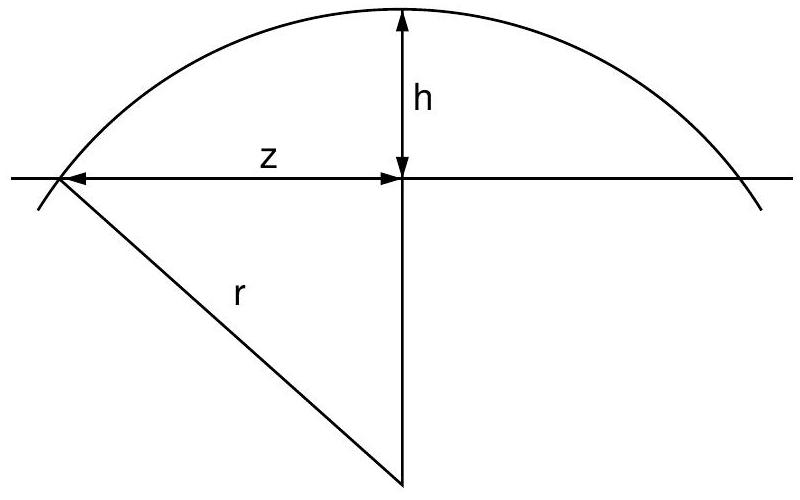
\includegraphics[width = 0.95\linewidth, center]{2024_12_03_2b013636ff75d184213cg-6}
	\caption{Určení poloměru křivosti kulové plochy.}
\end{figure}



\section*{Měření křivosti lámavých ploch sférometrem}

Poloměry křivosti lámavých ploch $r_{1}$ a $r_{2}$ určíme sférometrem.  Hodinkový indikátor s přesností čtení rozdílu výšek $\pm 0,001 \mathrm{~mm}$ je upevněn v držáku s kruhovou základnou, jehož středem prochází dotykové čidlo. Nulovou polohu sférometru určíme tak, že jej umístíme na rovinné sklo. Pak postavíme sférometr na měřenou kulovou plochu s poloměrem křivosti $r$. Je zřejmé, že kruhová základna sférometru s poloměrem z vytne na povrchu měřené plochy kulovou úseč s výškou $h$. Rozdíl údajů sférometru na čočce a na rovinném skle právě udává tento parametr. Změříme-li průměr sférometru $2 z$ posuvným měřítkem, pak zřejmě

\begin{equation}
	r=\frac{z^{2}+h^{2}}{2 h}
\end{equation}



	
		\section{Měření}
		\subsection{Ohnisková vzdálenost spojky}		
		Z měření získáváme:\\ \\
		{\small \begin{tabular}{rrrr|rrr}
			
			a[cm] & a'[cm] & Beta & $\Delta$[cm] & f'[cm] & $f_2^\prime$[cm] & $f_B^\prime$[cm] \\
			
			-20.75 & 71.40 & -3.30 & 49.00 & 16.08 & 15.92 & 16.52 \\
			-21.30 & 66.70 & -3.00 & 43.50 & 16.14 & 15.98 & 16.62 \\
			-21.60 & 62.40 & -2.76 & 39.10 & 16.05 & 15.86 & 16.45 \\
			-22.50 & 57.50 & -2.43 & 33.25 & 16.17 & 15.94 & 16.55 \\
			-23.45 & 52.55 & -2.13 & 27.35 & 16.21 & 15.96 & 16.54 \\
			-24.85 & 47.15 & -1.81 & 21.00 & 16.27 & 16.01 & 16.47 \\
			-25.00 & 46.00 & -1.77 & 19.00 & 16.20 & 15.97 & 16.48 \\
			-26.40 & 42.60 & -1.55 & 14.80 & 16.30 & 16.05 & 16.46 \\
			-26.65 & 41.35 & -1.48 & 12.40 & 16.21 & 15.90 & 16.43 \\
			-34.25 & 33.65 & -1.00 & 0.00 & 16.97 & 17.12 & 16.98 \\
			
			
		\end{tabular}}
	\begin{align*}
		f^\prime = 16.26 \pm 0.26 \,\mathrm{cm}, \\ f_2^\prime = 16.1\pm 0.4 \,\mathrm{cm}, \\ f_B^\prime = 16.55 \pm 0.19 \,\mathrm{cm}
	\end{align*}
	\subsection{Ohnisková vzdálenost rozptylky}
	Získáváme:\\
	
\begin{tabular}{rrrrr|r}

	 A[cm] & A'[cm] & R[cm] & a[cm] & a'[cm] & f'[cm] \\
	
	 69.85 & 96.10 & 52.50 & 17.35 & 43.60 & -28.82 \\
	 69.85 & 92.70 & 53.20 & 16.65 & 39.50 & -28.78 \\
	 69.85 & 91.25 & 53.60 & 16.25 & 37.65 & -28.59 \\
	 69.85 & 89.15 & 54.00 & 15.85& 35.15 & -28.87 \\
	 69.85 & 88.00 & 54.65& 15.20& 33.35 & -27.93 \\
	 69.85 & 86.50 & 55.00 & 14.85 & 31.50 & -28.09 \\
	 69.85 & 85.00 & 55.80 & 14.05 & 29.20 & -27.08 \\
	 69.85 & 82.00 & 56.50 & 13.35 & 25.50 & -28.02 \\
	 69.85 & 80.00 & 57.85 & 12.00 & 22.15 & -26.19 \\
	 69.85 & 78.00 & 58.75 & 11.10 & 19.25 & -26.22 \\
	
\end{tabular}
\begin{equation*}
	f^\prime = -27.9\pm 1.0
\end{equation*}
\subsection{Měření křivosti}

Sférometrem o poloměru \\$z = 17.477 \pm 0.007 \,\mathrm{mm}$ získáváme:

\begin{tabular}{ccc}
	& spojka               & rozptylka       \\
	$h1$[mm] & $1.833 \pm 0.0003  $   & $0.508\pm 0.0003 $\\
	$h2$[mm]& $0.0001 \pm 0.0002 $   & $0.507\pm 0.0004$ \\
	$r1$[mm] & $334.19\pm 0.29   $    & $300.89\pm 0.31$  \\
	$r2$[mm] & $6.1 \pm 1.2 .10^{-5} $& $-301.48\pm 0.35$ \\ \hline
$	n$  & $1.514 \pm 0.008 $     & $1.540\pm 0.019 $
\end{tabular}
		
		\section{Závěr}
		Podařilo se nám splnit veškeré zadané úkoly a získat hodnoty hledaných veličin. Je třeba myslet na to, že skutečné hodnoty nevíme, všechny hodnoty však vypadají realisticky a při měření stejné veličiny různými metodami si jsou též velmi blízké
		
	
		

		
		
		
		
		
		% Nakonec nezapomeňte projet text programem vlna nebo vlnka, např.
		% 	vlna -m -l -n mojeuloha.tex
		% nebo zkontrolovat a opravit jednopísmenné předložky na koncích řádků ručně.
	\end{multicols}
\end{document}
